%%%%%%%%%%%%%%%%%%%%%%%%%%%%%%%%%%%%%%%%%%%%%%%%%%%%%%%%%%%%%%%%%%%%%%%%%%%%%
\section{OpenCL and Device Fission}

OpenCL consists of an API for coordinating \textit{parallel computation across heterogeneous processors} (CPU, GPU and other processors) and it is supported by a wide range of systems and platforms, making it the perfect choice for parallel computation not only on traditional desktop CPU-GPU configuration, but also on embedded systems.


%-----------------------------------------------------------------------------
\subsection{OpenCL Architecture}

%OpenCL is a framework which is composed of 4 main components:
%
%\begin{enumerate}
%	\item a \textbf{language} [APPROFONDIRE]
%	\item an \textbf{API} [APPROF]
%	\item a series of \textbf{libraries} [APPROF]
%	\item a \textbf{runtime system} [APPROF]
%\end{enumerate}
%
%To better describe the architecture of OpenCL, we can divide it into four models:
%
%\subsubsection{The Platform Model}
We can define the structure of an OpenCL application by defining its components. Some of these components are purely abstract and refer to the "`software"' part of the application (the host), devices mixes both software and hardware abstraction, while Compute Units and Processing Elements are direct references to the graphic hardware.

\begin{itemize}
	\item the \textbf{Host} can be viewed as the "`outer control logic"' of the application. It is usually executed on the CPU and its function is to configure the application accordingly to the architecture of the hosting machine, and to submit commands to the computing units.
	\item one or more \textbf{OpenCL Devices} connected to the host. These devices can be physical (e.g. the graphic adapter installed on the system) or virtual (e.g. remote GPUs in a cluster configuration - for more info about OpenCL clustering refer to the VCL project, http://wwww.mosix.org)
	\item various \textbf{Compute Units} (CU) that are the equivalent of CUDA's Stream Multiprocessors introduced in \textbf{Figure} \ref{fig:scalability}.
	\item each Compute Unit is divided into several \textbf{Processing Elements} (PE). Each PE can work both in \textbf{SIMD} mode (Single Instruction Multiple Data), therefore exploiting \textit{data level parallelism} and \textbf{SPMD} mode (Single Program Multiple Data): the program is divided into independent task that are executed simultaneously.
\end{itemize}

The architecture of an OpenCL application is summarized in \textbf{Figure} \ref{fig:OpenCLArch}:

\begin{figurehere}
 \centering
 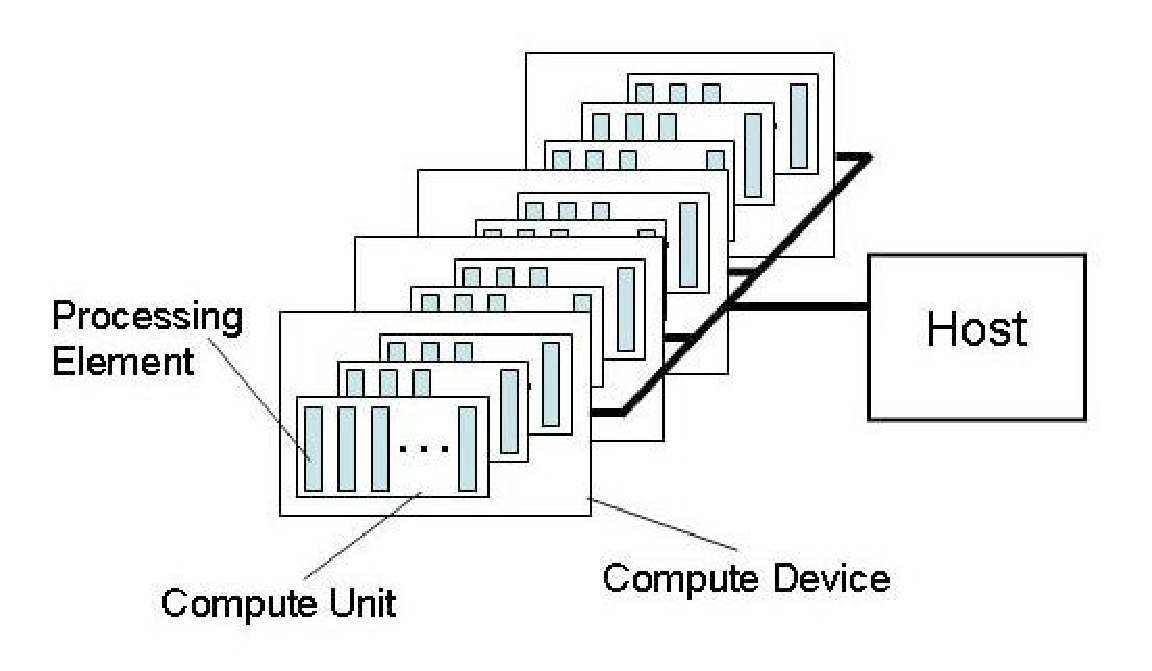
\includegraphics[width=8cm, height=4cm]{./eps/OpenCLArch.eps}
 \caption{OpenCL Architecture}
 \label{fig:OpenCLArch}
\end{figurehere}

\subsubsection{Execution and Index Space}

From a very coarse point of view, we can describe the execution of an OpenCL application as a two-step process:

\begin{enumerate}
	\item the \textbf{host} define the context for \textbf{kernels} and submit them for execution.
	\item the \textbf{kernel} executes on one or more OpenCL device and compute over a stream of data.
\end{enumerate}

In OpenCL, an instance of a kernel is called \textbf{work-item} and it executes over an \textbf{index-space} that is defined every time a new kernel is submitted. We can see the index space as the data domain over which the multiple instances of a kernel may work, and it is also called \textbf{NDRange} (N-dimensional index space, where N is one, two or three). From the graphical point of view of the GPU computation, the index range is no more than the texture on which apply the shader (in fact GPUs normally support 1,2 or 3-dimensional textures).\\

\begin{figurehere}
 \centering
 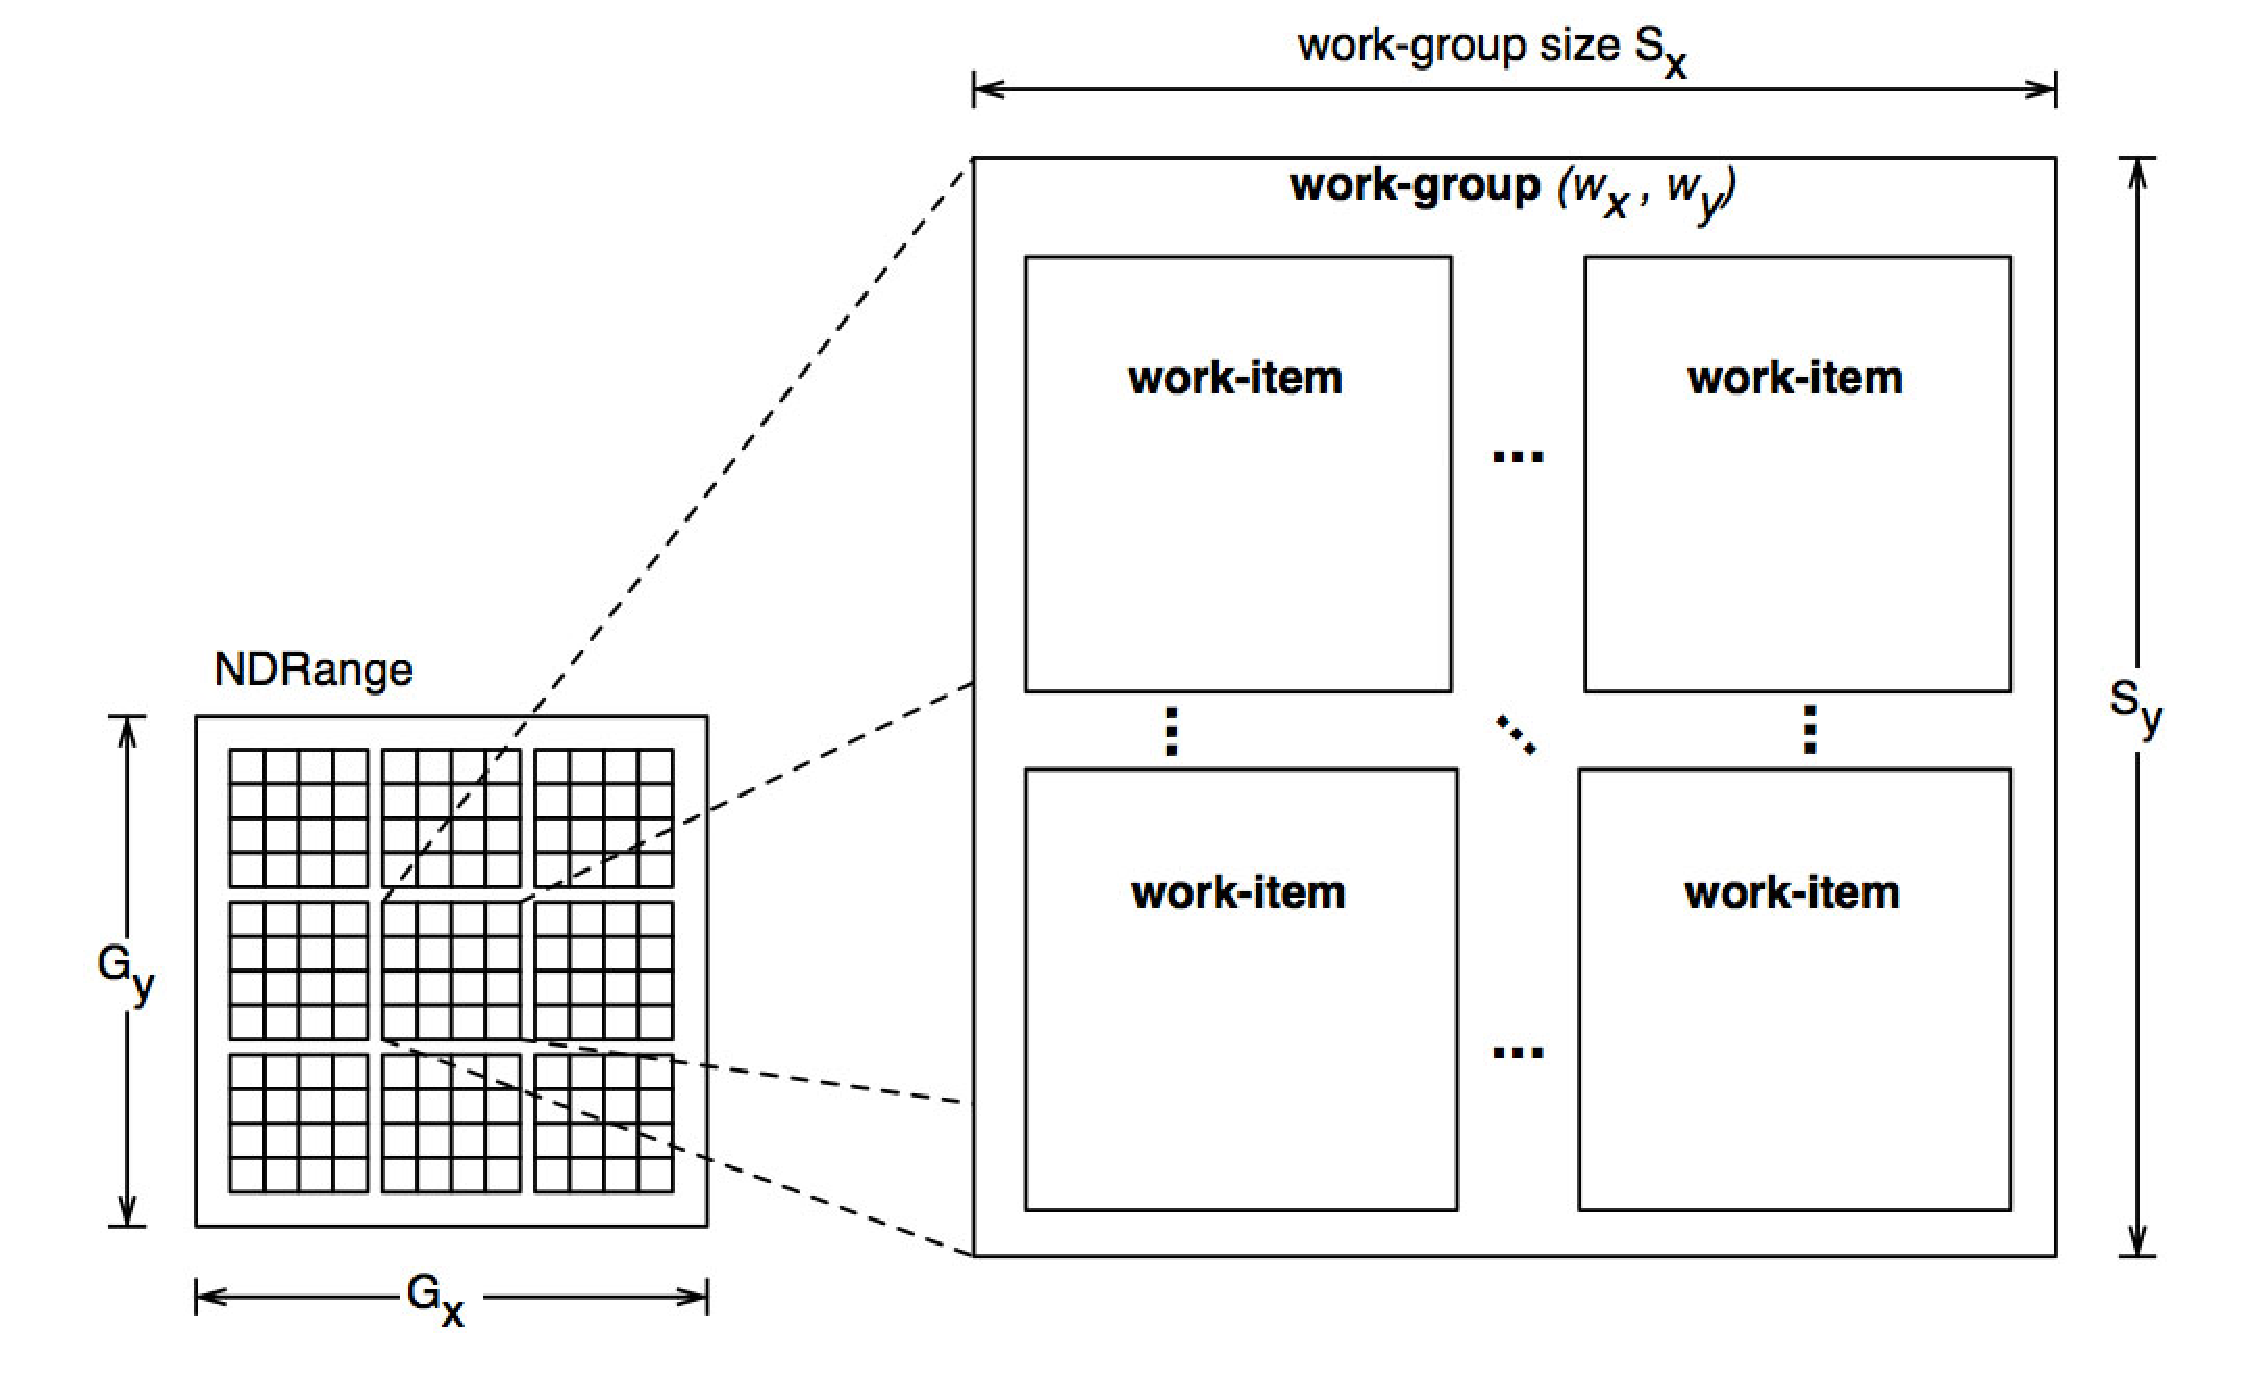
\includegraphics[width=8cm, height=4cm]{./eps/index-space.eps}
 \caption{Work-items mapped over a 2-D NDRange. As you can see, work-items can be organized in Work-Groups. Every work-item has both global and local IDs inside its work-group.}
 \label{fig:indexSpace}
\end{figurehere}

\subsubsection{Program Context and Command-Queue}

When the host defines the \textbf{context} for the application, it basically define four things:

\begin{enumerate}
	\item the collection of OpenCL devices to be used
	\item the collection of functions that will be executed on the devices (that is, the kernels)
	\item \textbf{program objects}, that are simply the source files and executables that implements the kernels
	\item \textbf{memory objects}: the data to be computed
\end{enumerate}

After the context has been created, the host initialize a structure called \textbf{command queue} that is used to schedule commands onto the devices within the context. The command structure is very simple and the main commands issued by the host are only three:

\begin{enumerate}
	\item \textbf{Kernel execution commands}: Execute a kernel on the PEs (Processing Elements) of a device
	\item \textbf{Memory commands}: Transfer data to, from, or between memory objects, or map and unmap
memory objects from the host address space.
	\item	\textbf{Synchronization commands}: Used to specify the order of execution of commands.
\end{enumerate}

\subsubsection{Memory}

There are four types of memory regions in OpenCL: \textbf{Global}, \textbf{Constant}, \textbf{Local} and \textbf{Private}.

\begin{itemize}
	\item Global memory grants read/write access to \textbf{all} the work-items in every work-group.
	\item Constant memory is only used to store constants. Only the host has write privileges over it, while kernels can only read from it.
	\item Local memory is shared among all the work-items that form a group. The host has no access to this memory.
	\item Private memory is allocated directly by the work-item and can be used only by itself. The host has no access to this part of memory.
\end{itemize}

Since computation is carried on parallely, one of the major issues about memory is \textbf{consistency}. OpenCL uses a relaxed consistency memory model: the state of memory visible to a work-item is not guaranteed to be consistent across the collection of work-items at all times. \textbf{Table} \ref{tab:memconsistency} summarizes memory consistency for the various regions of memory available.\\

\begin{tablehere}
{\footnotesize
\begin{tabular}{|p{2cm}|p{5,5cm}|} \hline
\textbf{Memory} & \textbf{Consistency}\\ \hline
Private & memory is not shared, read/write consistency is always guaranteed\\ \hline
Local & consistency is guaranteed between work-items of the same work-group\\ \hline
Global & consistency is guaranteed between work-items of the same work-group, but not between multiple work-groups in the case they are assigned to execute the same kernel\\ \hline
\end{tabular}}
\caption{Memory consistency}
\label{tab:memconsistency}
\end{tablehere}


In OpenCL computation is performed over \textbf{memory objects}. There are two distinct memory objects: \textbf{buffers} and \textbf{images}.

\begin{itemize}
	\item Buffers are used to store a one-dimensional collection of elements (like an array), and those elements can be scalar values (int, float, etc.), vectors or user defined structures.
	Buffers are stored sequentially and \emph{can be accessed using pointers}; elements of a buffer are stored in memory in the \emph{same format} as they are used by kernels (i.e. if the kernel works on single integers, these elements are stored in memory as integers, this is not true for image objects)
	\item Images are used to store bi- or three-dimensional structures and their elements cannot be only selected by a list of predefined image formats (i.e. you cannot simply declare int or floats in an image object). Differently from buffers, elements of images \emph{cannot be accessed directly with a pointer} and they are \emph{always stored in memory as 4-dimensinal vectors} (since graphic shaders work on RGB and Alpha components of the pixels of an image)
\end{itemize}

\begin{CLCode}
In OpenCL memory objects are stored into \textbf{cl\_mem} structs, that can be easily initializated with the \textbf{clCreateBuffer()} and \textbf{clCreateImage()} functions.\\
Image format availables may vary from one graphic adapter to another, a list of supported image formats can be obtained using the \textbf{clGetSupportedImageFormats()} query.
\end{CLCode}

















%-----------------------------------------------------------------------------
\subsection{The second subsection of the second \\ Section}

Lorem ipsum dolor sit amet, consectetur adipiscing elit. Mauris eget mauris.
Nulla facilisi. Ut condimentum tempor eros? Integer metus mauris, consectetur
sit amet, tempor a, facilisis eu, nisl. Vestibulum at turpis. Ut vitae tortor
pretium nisl vestibulum blandit. Nulla nibh urna, semper et, elementum at,
mattis ut, nisi! Cum sociis natoque penatibus et magnis dis parturient montes,
nascetur ridiculus mus. Morbi vel ligula eget lacus convallis venenatis. Aliquam
lacinia tincidunt felis. Ut dui.
